\lecture{9}{2025-03-15}{Limite est continuité}{}
\begin{parag}{Rappel}
    \begin{definition}
        Soit $E \subset \mathbb{R}^n $ sous-ensemble non vide, $n \geq 1$ Une fonction est une application qui envoie chaque point $ \overline{x0} = (x_1, \dots, x_n) \in E$ dans $ \mathbb{R}$.\\
        $E$ est le domaine de définition de $f$ et $f(E) \subset \mathbb{R}$ est l'ensemble image.
    \end{definition}
    

\end{parag}

\subsection{Limites et continuité}
\begin{definition}
    Une fonction \important{définie au voisinage de $\overline{x_0}$} (mais pas nécéssairement en $ \overline{x_0}$ tel que
    \begin{align*}
        [ \exists \delta > 0: B( \overline{x}_0, \delta) \subset E \cup \{ \overline{x_0}\}]
    \end{align*}
    admet pour \important{limite} le nombre réel $l$ lorsque $ \overline{x}$ tend vers $ \overline{x_0}$ si \important{pour tout $ \epsilon > 0 \exists \delta > 0$ tel que pour tout $ \overline{x}\in E$ et $0 < \mid \mid \overline{x} - \overline{x}_0 \mid \mid \leq \delta$,  on a $ \mid f( \overline{x}) - l \mid \leq \epsilon$} 
\end{definition}


 \begin{parag}{Notation}
     Pour notre notation on utilise comme à notre habitude:
     \begin{align*}
         \lim_{ \overline{x} \to \overline{x_0}}f( \overline{x}) = l
     \end{align*}
     \begin{framedremark}
         Ici on a la norme $  \mid \mid \overline{x} - \overline{x_0} \mid \mid$ à la place de la valeur absolue lorsqu'on parlait de fonction à une variable. 
     \end{framedremark}
     
 \end{parag}
 \begin{parag}{Continuité}
 
 
 \begin{definition}
     Soit $ \overline{x_0} \in E$ un point intérieur de $E$. Alors $f: E \to \mathbb{R}$ est continue en $ \overline{x} = \overline{x_0}$ \important{si et seulement si}
     \begin{align*}
     \lim_{ \overline{x} \to \overline{x_0}} f( \overline{x}) = f( \overline{x_0})
     \end{align*}
     
 \end{definition}
 

 \begin{subparag}{Exemple 1}
     \begin{align*}
         f(x, y) = 2x + y
     \end{align*}
     soit $(x_0, y0) \in \mathbb{R}^2$: Alors 
     \begin{align*}
         \lim_{(x, y) \to (x_0, y_0)} (x + 2y) = x_0 + 2y_0
     \end{align*}
     Soit $ \epsilon > 0$ alors on cherche $ \mid f(x, y) - f(x_0, y_) \mid = \mid  (x + 2y) - (x_0 + 2y_0) \mid$ si on utilise plus la norme ici et la valeur absolue car on est sur le côté à droite. On utilise l'inéégalité triangulaire:
     \begin{align*}
        &\leq \mid x - x_0 \mid + 2 \mid y - y_0 \mid
     \end{align*}
     Ici on peut toujours prendre comme on a que $ \overline{x} - \overline{x_0}$ plus petit que $ \delta$ on doit les gérer ensembles et non séparément. Des lors:
     Dès lors on choisit $ \delta = \frac{ \epsilon}{3}$
        \begin{align*}
        \leq \sqrt{ (x-x_0)^2 + (y-y_0)^2} + 2\sqrt{(x-x_0)^2 + (y-y_0)^2} = 3\sqrt{(x -x_0)^2 + (y-y_0)^2} \leq 3 \delta = 3 \cdot \frac{ \epsilon}{3} = \epsilon
           \end{align*}

 \end{subparag}
 \begin{subparag}{Exemple 2}
     \begin{align*}
         f(x, y) = x \cdot y \\
         f: \mathbb{R}^2 \to \mathbb{R}
     \end{align*}
     Soit $(x_0, y_0) \in \mathbb{R}^2$ Alors $ \lim_{(x, y) \to (x_0, y_0)} x \cdot y = x_0 \cdot y_0$
     
     \textbf{Démonstration:}\\
    Le cas où $x_0 = 0$ est vu en exercice, dès lors, nous traiterons ici le cas où nous supposerons que $x_0 \neq 0$. Soit $ \epsilon > 0$ alors:
    \begin{align*}
        \mid f(x, y) - f(x_0, y_0)\mid &= \mid xy - x_0y_0 \mid  \\
        &= \mid  (x - x_0)y + x_0(y-y_0) \mid\\
        &\leq \mid x-x_0 \mid \cdot \mid y \mid + \mid y-y_0 \mid \cdot \mid x_0 \mid\\
        \mid y - y_0 \mid \cdot \mid x_0\mid \leq \sqrt{ (x-x_0)^2 + (y-y_0)^2} \mid x_0 \mid \leq  \frac{ \epsilon}{2} \implies \delta \leq \frac{ \epsilon}{2 \mid x_0 \mid} (x_0 \neq 0)\\
        \mid x - x_0 \mid y \mid\mid \leq \sqrt{ (x-x_0)^2 + (y-y_0)^2}\cdot \mid y \mid \leq  \delta  ( \mid y_0 \mid + \delta) \leq \frac{ \epsilon}{2}\\
        \leq \frac{ \epsilon}{2}\\
        \implies \delta \leq \frac{ \epsilon}{2( \mid y_0 \mid + 1)}
    \end{align*}
    On peut choisir comme valeur pour $ \delta$:
    \begin{align*}
        \implies \delta = \text{min} \left( \frac{e}{2 \mid x_0 \mid}, \frac{ \epsilon}{2( \mid y_0\mid + 1)} , 1 \right)  \implies \mid f(x, y)  f(x_0, y_0) \mid \leq \frac{ \epsilon}{2} + \frac{ \epsilon}{2} = \epsilon
    \end{align*}
    
    
     
 \end{subparag}
 \end{parag}

 \begin{parag}{Caractérisation de la limite à partir des suites convergentes}
     \begin{theoreme}
         Une fonction $f: E \to \mathbb{R}$ définie au voisinage de $ \overline{x_0}$ admet pour limite $l \in \mathbb{R}$ lorsque $ \overline{x} \to \overline{x_0}$  \important{Si et seulement si} pour toute suite d'élément $\{ \overline{a_k}\}$ de $\{ \overline{x} \in E: \overline{x} \neq \overline{x_0}\}$, qui converge vers $ \overline{x_0}$, la suite $\{f( \overline{a}_k)\}$ converge vers $l$.
         \begin{align*}
             \lim_{ \overline{x} \to \overline{x_0}} f( \overline{x}) = l \iff \lim_{ k \to \infty} f( \overline{a_k}) = l \text{ pour toute suite } \{ \overline{a_k}\} \subset E \setminus \{ \overline{x_0}\}: \lim_{k \to \infty} \overline{a_k} = \overline{x_0}
         \end{align*}
     \end{theoreme}
 \end{parag}
 
 \begin{parag}{Démonstration}
     \begin{subparag}{ $ \implies$ $P \implies Q$}
         Comme ce théorème est une équivalence, nous allons devoir prouver les deux sens. Commençons par $P \implies Q$. Prenons la définition de la limite à gauche:
         \begin{align*}
             &\lim_{ \overline{x} \to \overline{x_0}} f( \overline{x})= l \implies \forall \epsilon > 0 \exists \delta > 0: \forall \overline{x}: 0 < \mid \mid \overline{x} - \overline{x_0} \mid \mid \leq \delta\\
             &\implies \mid f( \overline{x}) - l \mid \leq \epsilon \\
             &\text{Si on a } \{ \overline{a_k}\}: \lim_{k \to \infty} \overline{a_k} = \overline{x_0} \implies \text{  pour } \delta > 0 \exists k_0 : \forall k \geq k_0 \\
             &\implies \mid \mid \overline{a_k} - \overline{x_0} \mid \mid \leq \delta \implies \mid f( \overline{a_k}) - l \mid \leq \epsilon \\
             &\mid  f( \overline{a}_k) - l \mid \leq \epsilon
         \end{align*}
         \begin{framedremark}
             L'idée ici est de prendre le même $ \delta$ sur les deux première lignes.
         \end{framedremark}
         
     \end{subparag}
     \begin{subparag}{$(\impliedby)$ par contraposée}
         Petit rappel pour la contraposée: si on a $ Q \implies P$ alors la contraposé est $ \neg P \implies \neg Q$ donc ici on veut prouver que si la limite n'est pas $l$ alors la limite de $f( \overline{a_k})$ n'est pas non plus $l$.\\
         Supposons donc que $\lim_{ \overline{x} \to \overline{x_0}}f( \overline{x}) \neq l $ Alors:
             \begin{align*}
                 \exists \epsilon > 0: \forall \delta > 0 \exists \overline{x}_\delta: \mid \mid \overline{x_k} - \overline{x_0} \mid \mid \leq \frac{1}{ \delta} \mid \text{ et } \mid f( \overline{x}_\delta) - l \mid > \epsilon
             \end{align*}
             Dès lors, on peut choisir $ \delta = \frac{1}{k}$, $k \in \mathbb{N}^*$  ce qui implique:
             \begin{align*}
                 \exists \overline{x}_k \in E : \mid \mid  \overline{x_k} - \overline{x_0} \mid \mid \leq \frac{1}{k} \text{ et } \mid f( \overline{x_k}) - l \mid > \epsilon
             \end{align*}
             On obtient la suite $\{ \overline{x}_k\}_{k=1}^\infty: \lim_{k \to \infty} \overline{x_k} = \overline{x_0}$ mais $ \mid f( \overline{x_k}) - l \mid > \epsilon \forall k \in \mathbb{N}^*$ Dès lors
             \begin{align*}
                 \implies f( \overline{x}_k) \neq l
             \end{align*}
     \end{subparag}

     \begin{subparag}{Idée générale de la preuve}
         Ici on prends $P$ et \important{Ensuite} $\neg P$ il est important de pouvoir différencier les deux et de pouvoir construite $\neg P$ à partir de $P$.
         
     \end{subparag}
 \end{parag}

 \begin{parag}{Opération algébrique}
     Soit $f, g$ deux fonctions: $ E_{ \mathbb{R}^n } \to \mathbb{R}$ telles que $\lim_{ \overline{x} \to \overline{x_0}}f( \overline{x}) = l_1$ et $\lim_{ \overline{x} \to \overline{x_0}}g( \overline{x}) = l_2$ Alors:
     \begin{enumerate}
         \item $\lim_{ \overline{x} \overline{x_0}} ( \alpha f + \beta g)( \overline{x}) = \alpha l_1 + \beta l_2$
         \item $\lim_{ \overline{x} \to \overline{x_0}} (f \cdot g)( \overline{x}) = l_1 \cdot l_2$ 
         \item Si $l_2 \neq 0$, alors $\lim_{ \overline{x} \to \overline{x_0}}( \frac{f}{g})( \overline{x}) = \frac{l_1}{l_2}$
     \end{enumerate}
    \begin{subparag}{Conclusion}
        Tous les polynômes en plusieurs variables et toutes les fonctions rationnelles sont continues sur leur domaines de définition,
        \begin{framedremark}
            La caractérisation de la limite à partir des suites convergentes est pratique pour montrer qu'une fonction n'admet pas de limite en $ \overline{x_0} \in \mathbb{R}^n $.
        \end{framedremark}
    \end{subparag} 
    \begin{subparag}{Exemple 1}
        \begin{align*}
            f: \mathbb{R}^2 \to \mathbb{R}\\
            f(x, y) = \begin{cases}
                \frac{xy}{x^2 + y^2} \text{ si } (x, y) \neq (0, 0)\\
                0 \text{ si } (x, y) = (0, 0)
            \end{cases}
        \end{align*}
        Soit $ \overline{a_k} = ( \frac{1}{k}, \frac{1}{k}) \to (0, 0)$ qui implique donc pour la limite:
        \begin{align*}
            \lim_{ k \to \infty} f( \overline{a_k}) = \lim_{k \to\infty} \frac{ \frac{1}{k} \cdot \frac{1}{k}}{ \frac{1}{k^2} + \frac{1}{k^2}} = \frac{1}{2}
        \end{align*}
        Dès lors, on peut aussi prendre $ \overline{b_k} = ( \frac{1}{k},0) \to (0, 0)$ qui par le même procédé:
        \begin{align*}
            \lim_{k \to \infty} f( \overline{b_k}) = \lim_{k \to \infty} \frac{ 0 \cdot \frac{1}{k}}{0 + \frac{1}{k^2}} = 0
        \end{align*}
        Et donc, par la caractérisation à partir des suites, $\lim_{(x, y) \to (0, 0)} f(x, y)$ ne peut pas exister.\\
        On peut aussi prendre une autre suite du genre $ \overline{c_k} = ( - \frac{1}{k}, \frac{1}{k}) \implies \lim_{k \to \infty} f( \overline{a_k}) = - \frac{1}{2}$\\
        Alors quelle est la limite $f(x, y)$ en $(0, 0)$
         \begin{center}
     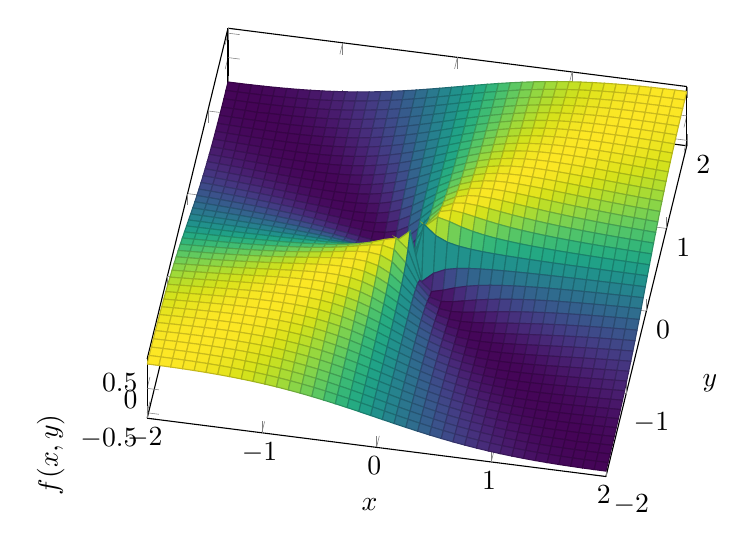
\begin{tikzpicture}
         \begin{axis}[
         view={10}{80},
         domain=-2:2,
         y domain = -2:2,
         colormap/viridis,
         xlabel={$x$},
         ylabel={$y$},
         zlabel={$f(x, y)$},
         samples=40,
         samples y=40,
         ]
         \addplot3[surf] {x*y/(x^2 + y^2)};
     \end{axis}
     \end{tikzpicture}
     
     
 \end{center}
 
    \end{subparag}
    \begin{subparag}{Proposition}
        \begin{theoreme}
            soir $D \subset \mathbb{R}^n $, $f: D \to \mathbb{R}$ définie au voisinage de $ \overline{x_0} \in \mathbb{R}^n $. Alors $\lim_{ \overline{x} \to \overline{x_0}}f( \overline{x}) =l$ si et seulement si pour toute courbe $ y: [a, b] \to \mathbb{R}^n $ telle que:
            \begin{align*}
                 \Upsilon([a, b]) \subset D \setminus\{ \overline{x_0}\} \text{ et } \lim_{t \to a^*} y(t) = \overline{x_0}, \text{ on a } \lim_{t \to a^+} f(y(t)) = l
            \end{align*}
           
        \end{theoreme}
       \begin{framedremark}
           On ne peut pas calculer la limite d'une fonction de plusieurs variable en faisant de manière consecutive par rapport à chaque variable.

       \end{framedremark}
        
    \end{subparag}

    \begin{subparag}{Exemple 2}
        \begin{align*}
            f(x, y) = \begin{cases}
                \frac{x^2 - y^2}{x^2 + y^2} \text{ si } (x, y) \neq (0, 0)\\
                0 \text{ si } (x, y) = (0, 0)
            \end{cases}
        \end{align*}
        Alors on prends deux fonctions;:
        \begin{align*}
            y_1(t) = (t, 0)\\
            y_2(t) = (0, t)
        \end{align*}
        \begin{align*}
            \lim_{t \to o}( \gamma_1(t)) = \lim_{t \to o} \frac{t^2 - 0}{t^2 + 0} = 1\\
            \lim_{t \to 0}f( \gamma_2(t)) = \lim_{t \to 0} \frac{0 - t^2}{0 + t^2} = -1
        \end{align*}
       Et donc la fonction n'a pas de limite en ce point.
    \end{subparag}
    \begin{subparag}{Exemple 3}
        soit:
        \begin{align*}
            f: \mathbb{R}^2 \to \mathbb{R}\\
            f(x, y) = \begin{cases}
                \frac{x^3 + y^3}{x^2 + y^2}\\
                0
            \end{cases}
        \end{align*}
        En prenant les mêmes fonctions:
        \begin{align*}
            \gamma_1(t) = (t, 0) \implies \lim_{t \to 0} \gamma_1(t) = \overline{0}, \lim_{t \to 0} \frac{t^3 + 0}{t^2 + 0} = 0\\
            \gamma_2(t) = (0, t) \implies \lim_{ t \to 0} \gamma_2(t) = \overline{0}, \lim_{t \to 0} \frac{0 - t^3}{0 + t^2} = 0\\
                    \gamma_3 (t, t) \implies\lim_{t \to 0} \gamma_3(t) = \overline{0}, \lim_{t \to 0} \frac{t^3 + t^2}{t^2 + t^1} = 0
        \end{align*}
       On voit ici que ces fonctions ont toute la même limite, et si on prenait n'importe quelle autre  fonction la limite existerait toujours.
       \textbf{Hypothèse} $\lim_{(x, y) \to (0, 0)} f(x, y) = \overline{0}$
    \end{subparag}
 \end{parag}
 
 \begin{parag}{Méthode de changement de variables polaires}
     On peut démontrer l'existence de cette limite par le changement de variables en coordonnées polaires.:
     \begin{align*}
         x = r\cos \phi \text{ si } r \in \mathbb{R}_{ \geq 0}\\
         y = r\sin \phi \text{ si } r \neq 0
     \end{align*}
     Alors on a:
     \begin{align*}
         f(x, y) &= \frac{x^3 + y^3}{x^2 + y^2} \implies f(r, \phi) = \frac{r^3\cos^3\phi + r^3\sin^3\phi}{r^2\cos^2\phi + r^2\sin^2\phi}\\
         &= \frac{r^2(cos^3\phi + \sin^3\phi)}{r^2}\\
         &= r(cos^3\phi + \sin^3\phi)
     \end{align*}
     Ici, $\phi(r)$ est une fonction inconnue, elle pourrait être n'importe quoi.
     \begin{align*}
         \lim_{(x, y) \to (0, 0)}f(x, y) = \lim_{r \to 0} \Phi(r, \phi)\\
         \lim_{r \to 0}\mid r (cos^3\phi + \sin^3\phi) \mid = 0\\
         \implies \lim_{(x, y) \to (0, 0)} f(x, y) = 0
     \end{align*}
     
     
     \begin{framedremark}
         Cette méthode est efficace pour montrer l'existence des limites pour des fonctions de seulement deux variables, et qui tendent vers $(0, 0)$ tel que $\lim_{(x, y) \to (0, 0)} f(x, y)$
     \end{framedremark}
     
     
 
 \end{parag}
\begin{parag}{Théorème des $2$ gendarme}
    \begin{theoreme}
        Soit $f, g, h: E^{\subset \mathbb{R}^n } \to \mathbb{R}$ telles que:
        \begin{enumerate}
            \item $\lim_{ \overline{x} to \overline{x_0}}f( \overline{x}) = \lim_{ \overline{x} \to \overline{x_0}} g( \overline{x}) = l$
            \item Il existe $ \alpha > 0$ pour tout $x \in \{ x \in E: o < \mid \mid \overline{x}- \overline{x_0} \mid \mid \leq \alpha\}$ on a:
                \begin{align*}
                    f( \overline{x}) \leq h( \overline{x}) \leq g( \overline{x})
                \end{align*}
       Alors:
       \begin{align*}
           \lim_{ \overline{x} \to \overline{x_0}}h( \overline{x}) = l
       \end{align*}
        \end{enumerate}
    \end{theoreme}
    
\end{parag}
 
\begin{parag}{Critère des $2$ gendarmes en coordonnées polaires}
    \begin{subparag}{Proposition}
        Soit $D \subset \mathbb{R}^2, f: D \to \mathbb{R}$ définie au voisinage de $(x_0, y0) \in \mathbb{R}^2$. \\
        Alors
        \begin{align*}
            \lim_{(x, y) \to (x_0, y_0)} f(x, y) = l \text{ si et seulement si}
        \end{align*}
      \begin{align*}
          \exists \delta > 0 \text{ et } \phi: ] 0 , \delta [ \to \mathbb{R}:
      \end{align*}
    \begin{itemize}
        \item $ \forall \phi \in [0, 2\pi] \implies \mid f(x_0, r\cos\phi, y_0 + r\sin\phi) - l \mid \leq \phi(r)$
        \item $\lim_{r \to o^+} \phi(r) = 0$
    \end{itemize}    
    \end{subparag}

    \begin{subparag}{Exemple 5}
       soit 
       \begin{align*}
           f(x, y) = \begin{cases}
               \frac{4xy^2}{x^2 + y^2 + 3y^4} \\
               0
           \end{cases}\\
           f(r\cos\phi, r\sin\phi) = \frac{4r^3\cos\phi\sin^2\phi}{r^2 + 3r^4\cos^4\phi} = \frac{4r^3\cos\phi\sin^2\phi}{r^2(1 + 3r^2\sin^4\phi}\\
           \mid f(r\cos\phi, r\sin\phi) - 0 \mid = \frac{4r^3 \mid \cos\phi\sin^2\phi \mid}{r^2 \mid 1 + 3r^2\sin^4\phi \mid}
       \end{align*}
       On sait ici que la partie du nominateur (la partie en haut j'ai un doute) est toujours plus petite ou égale à 1 et la partie du bas plus grande ou égal à $1$. ce qui nous donne:
       \begin{align*}
           \leq \frac{4r^3}{r^2} = 4r = \Phi(r)
       \end{align*}
       Alors 
        \begin{align*}
            \lim_{r \to 0} \Phi(r) = 0
        \end{align*}
        Ce qui par les $2$ gendarmes en coordonnées polaires nous donne:
        \begin{align*}
            \lim_{(x, y) \to (0, 0)} f(x, y) = (0, 0)
        \end{align*}
    \end{subparag}
\end{parag}
\begin{parag}{Question à la fin du cours (Question 7)}
Soit les fonctions \begin{align*}
    f(x, y) = \begin{cases}
        \frac{cos(xy)(x^2 + \sin(y^2))}{\sqrt{x^2 + y^2}}, \; (x, y) \neq (0, 0)\\ 
        0 , \; \text{ Autrement}
    \end{cases} \\
    g(x, y) = \begin{cases}
        \frac{x^2 + y^4}{y^2 + x^4 + x^6}, \; \text{ si } (x, y) \neq (0, 0)\\
        0, \text{ autrement}
    \end{cases}
\end{align*}
La question est quelle fonction est continue en $(0, 0)$?
\begin{subparag}{Solution $f(x, y)$}
    On passe d'abord en coordonnées polaire:
    \begin{align*}
        f(r\cos\phi, r\sin\phi) = \frac{\cos(r^2\sin\phi\cos\phi)(r^2\cos\phi + \sin(r^2\sin^2\phi))}{r}
    \end{align*}
    On prend ensuite la limite:
    \begin{align*}
        \mid f(r\cos\phi, r\sin\phi) - 0 \mid &= \frac{ \mid \cos(r^2\sin\phi\cos\phi) \mid \mid r^2\cos\phi + \sin(r^2\sin^2\phi) \mid}{r}\\
                                              &\leq \frac{ \overbrace{r^2\cos\phi}^{ \geq r^2} + \mid \overbrace{\sin(r^2\sin^2\phi)}^{\leq \mid r^2\sin^2\phi \mid \leq r^2} \mid}{r}\\
                                              &\leq \frac{2r^2}{r} = 2r
    \end{align*}
    Et donc ici on voit que la limite de la fonction va bien vers $0$. ON peut aussi le \textit{"deviner}" en voyant un $r$ tout seul en bas et une $r^2\cos \dots$ en haut. Cela peut donner quelque indice.
\end{subparag}
\begin{subparag}{Solution $g(x, y)$}
    Pour cette fonction on refait le même procédé mais avant on va tester les limites du type $\lim_{t \to 0}g(0, t)$ et aussi $\lim_{t \to 0}g(t, 0)$ et on voit qu'elle ne donne pas la même réponse et que donc, la limite n'existe pas. 
    
\end{subparag}
\end{parag}


 
 
        
